\section{Polymer processing}
\label{chap1:sec:polymer_processing}

The polymer processing industry emerged in 1868~\cite{chap1:2002ebewele} and is nowadays an essential society sector, delivering many everyday items indispensable for a variety of purposes.
Polymeric materials, which include rubbers and plastics, have also stimulated major technological advance in many fields, for instance, health and transportation, among several others.
These materials present complex microscopic structures, leading to counter-intuitive physical properties, sometimes deviating significantly from the expected behaviour, typical of other common materials.
Consequently, the manufacturing technologies of polymeric materials have evolved into complex thermo-mechanical processes, and have been raising challenging problems for engineers, which require profound knowledge and experience.
The present section further explores the science and engineering behind polymeric materials, some manufacturing technologies, and some current and
emergent challenges.

\subsection{Polymers}
\label{chap1:subsec:polymer_processing_polymers}

Polymers are long molecular chains consisting of repetitive subunit molecules, having considerably lower molecular mass, referred to as monomers.
The chemical process of aggregating monomers together to form a polymer chain is referred to as polymerization, as exemplified in Figure~\ref{chap1:fig:polymer_processing_polymerization} for the case of the polystyrene, a polymer composed of styrene monomers.
Polymers obtained synthetically, based on oil or petroleum, are commonly referred to as plastics or rubbers.
In contrast, there is also a wide variety of polymers found in nature, usually denominated by biopolymers, such as cellulose, chitosan, genetic material, and carbohydrates.

\begin{figure}[!htb]
\centering
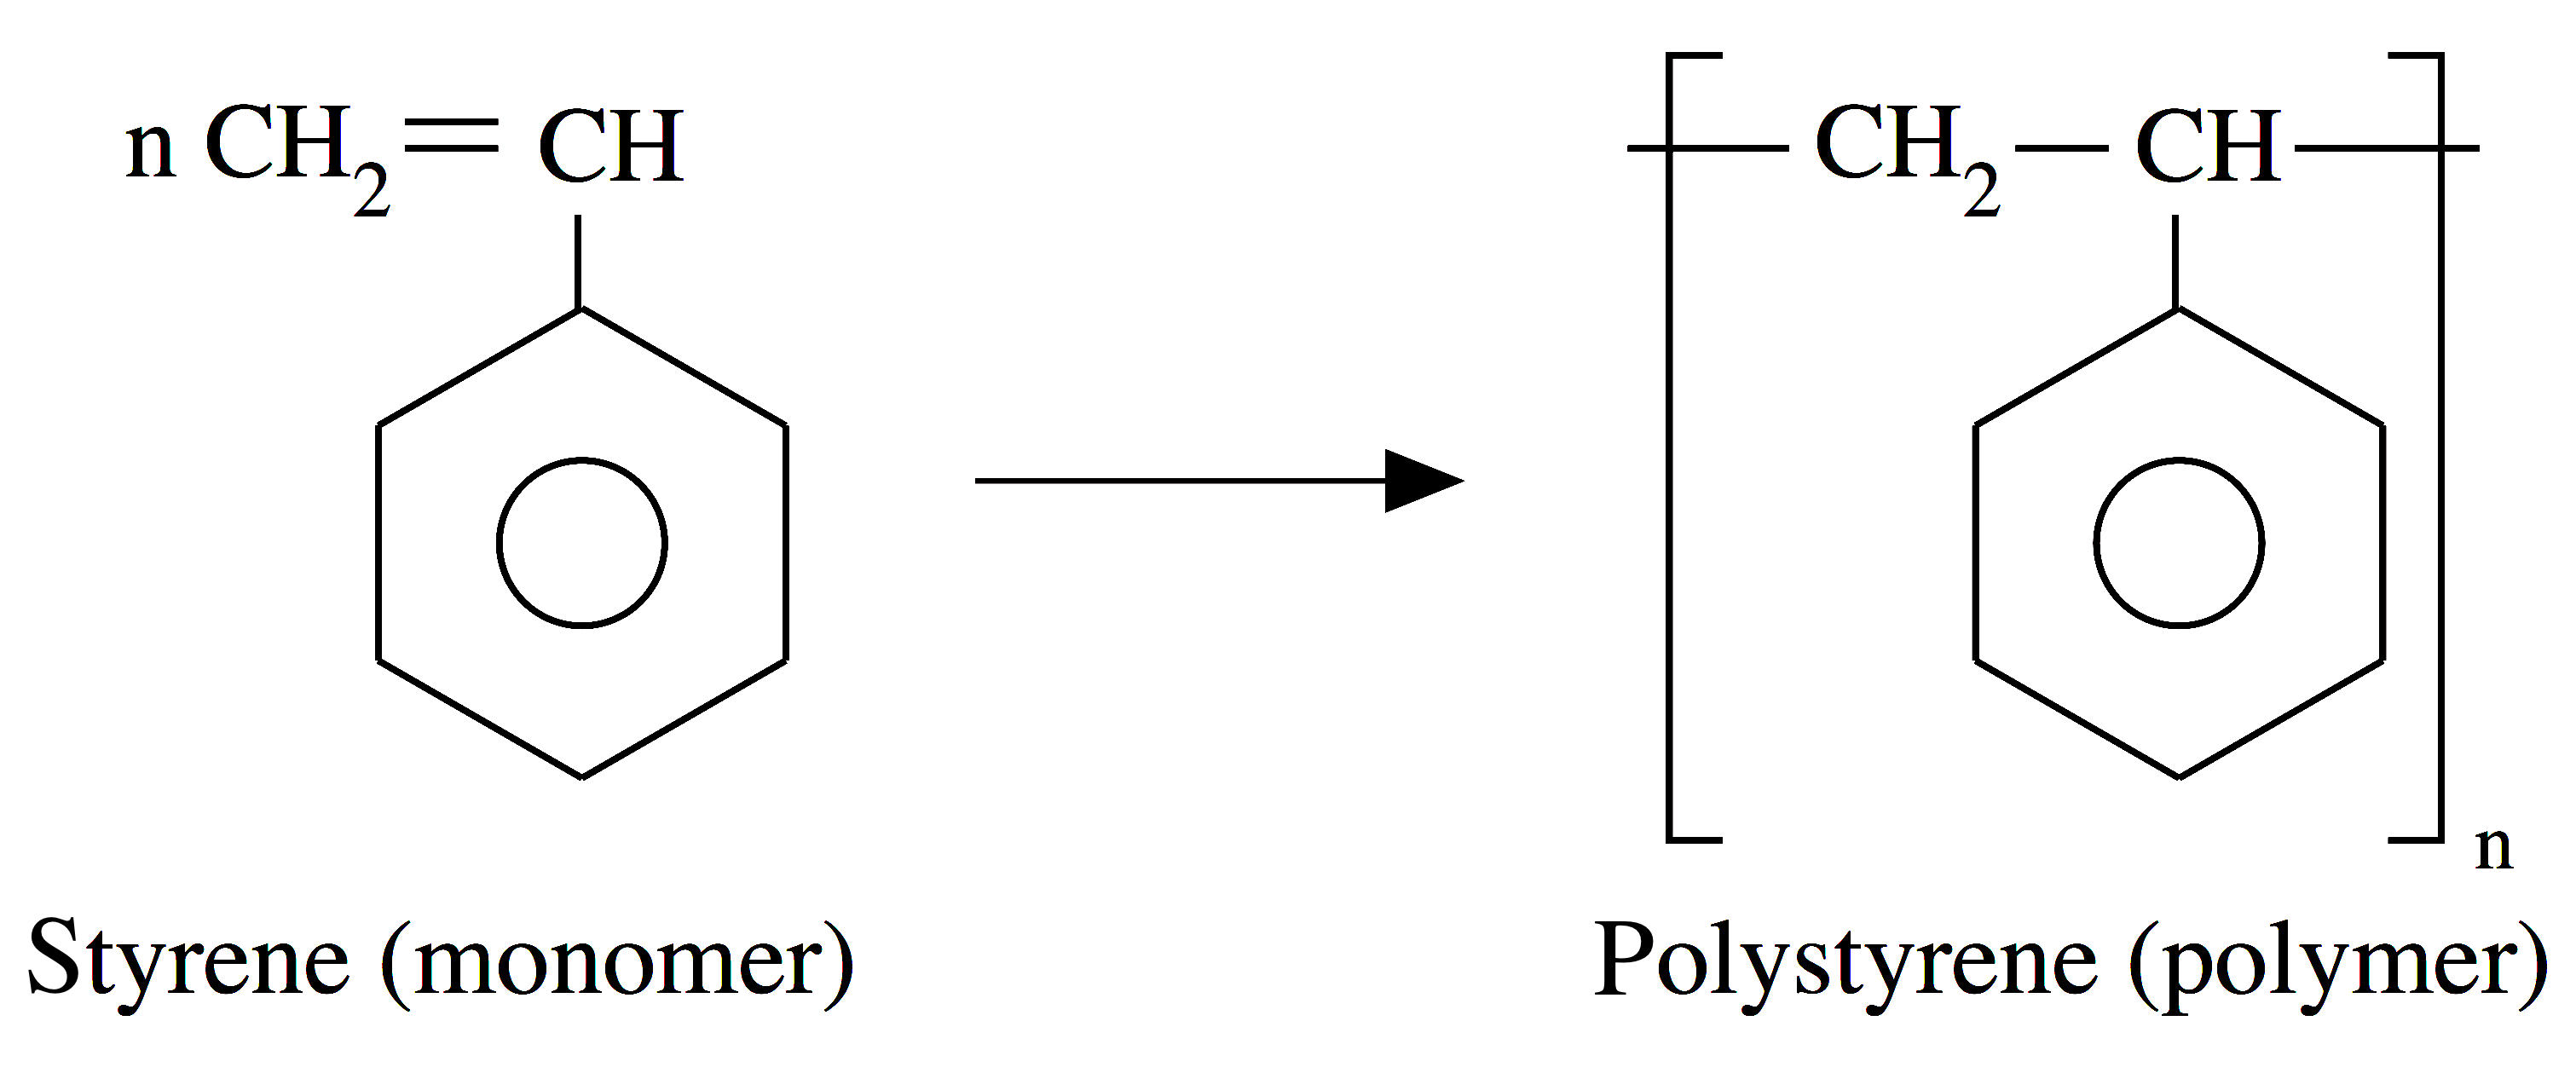
\includegraphics[width=0.5\textwidth]{chap1/include/figures/polymerization.png}
\caption[Polystyrene composed of styrene monomers.]{Polystyrene composed of styrene monomers (adapted from R.O. Ebewele, Polymer science and technology, CRC press, 2000).}
\label{chap1:fig:polymer_processing_polymerization}
\end{figure}

Polymers consisting of only one type of monomer are classified as homopolymers.
Otherwise, they are classified as copolymers, which in turn can be grouped according to the arrangement of the monomers in the polymer chain~\cite{chap1:2002ebewele} (random, alternating, block, and graft are the usual arrangements).
Polymers are also classified as unbranched, when consisting of a simple linear chain, or branched, when comprising a primary chain with one or more secondary side chains~\cite{chap1:2002ebewele}.
Moreover, polymers can also exhibit complex and intricate microscopic structures due to the arrangements of the chains, which can be chemically bonded, forming cross-linked structures.
In contrast, semi-crystalline structures form when individual chains are folded and packed regularly in three-dimensional arrangements, known as crystallites~\cite{chap1:2002ebewele}.
The microscopic arrangement of the chains, which are illustrated in Figure~\ref{chap1:fig:polymer_processing_microstructure}, strongly determines the materials physical properties.
In the solid-state, slightly cross-linked polymers tend to form elastomers, also referred to as rubbers, whereas highly cross-linked polymers tend to form thermoset plastics, which are irreversibly hardened.
On the other side, semi-crystalline polymers tend to form opaque materials, whereas amorphous polymers tend to be transparent.
In both cases, these polymers can be melted and solidified repeatedly, which justifies their group denomination as thermoplastics.
Molten thermoplastics also exhibit unique and, sometimes, counter-intuitive rheological properties, such as a combination of viscous and elastic behaviours, referred to as viscoelasticity.
Indeed, the viscosity is usually associated with fluids, whereas the elasticity is typically associated with solids.
The complexity of polymers has enabled the development of materials with advantageous physical properties, such as lightness and robustness, relevant for many technological fields, such as the transportation industry, health, construction, packaging, among many others.

\begin{figure}[!htb]
\centering
\begin{tabular}{@{}c@{}c@{}c@{}c@{}}

\includegraphics[width=0.25\textwidth]{chap1/include/figures/microstructure/microstructure-1.png}
& 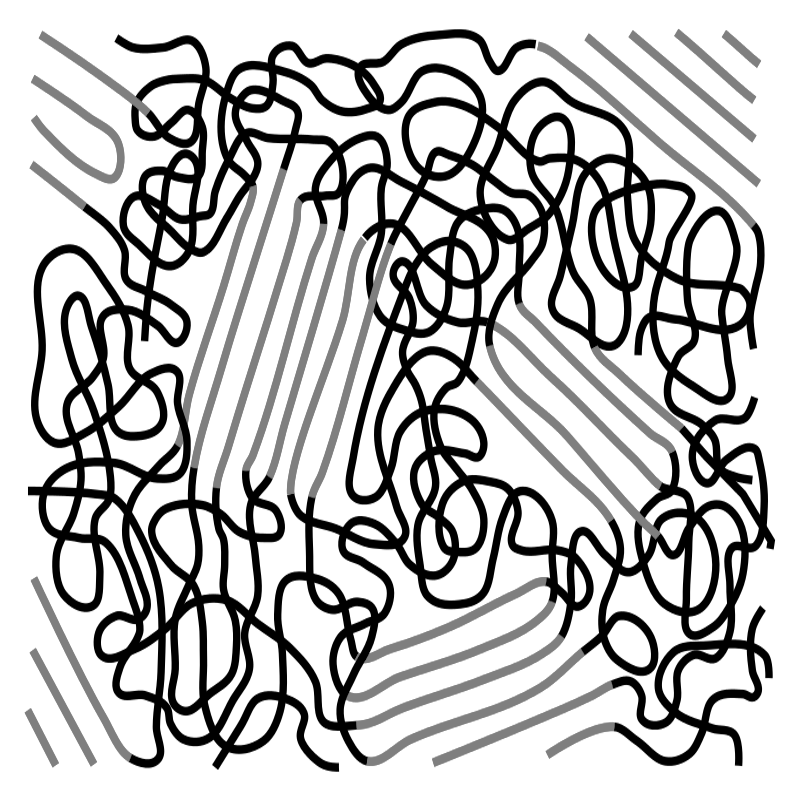
\includegraphics[width=0.25\textwidth]{chap1/include/figures/microstructure/microstructure-2.png}
& 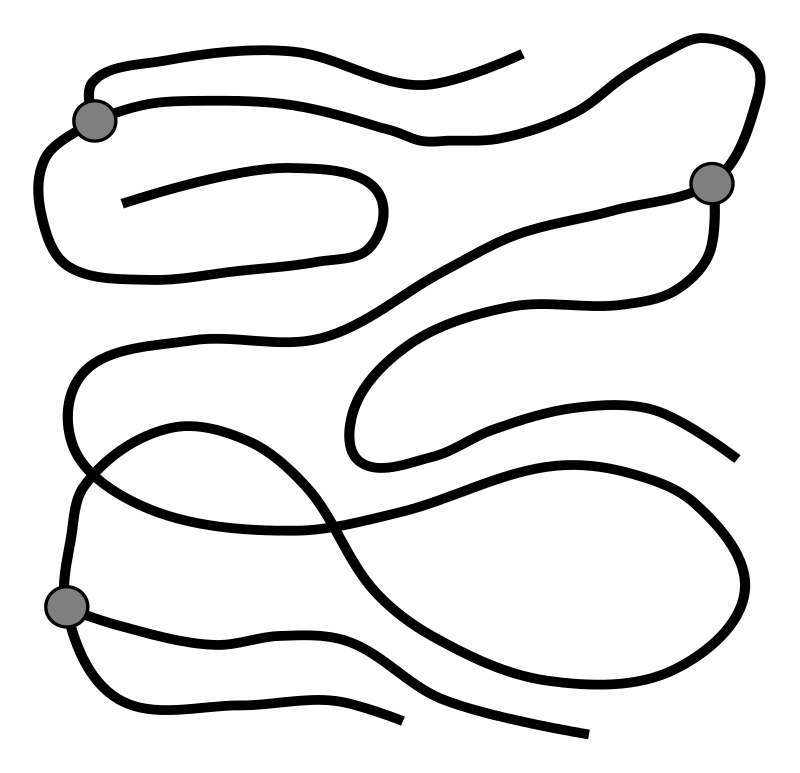
\includegraphics[width=0.25\textwidth]{chap1/include/figures/microstructure/microstructure-3.png}
& 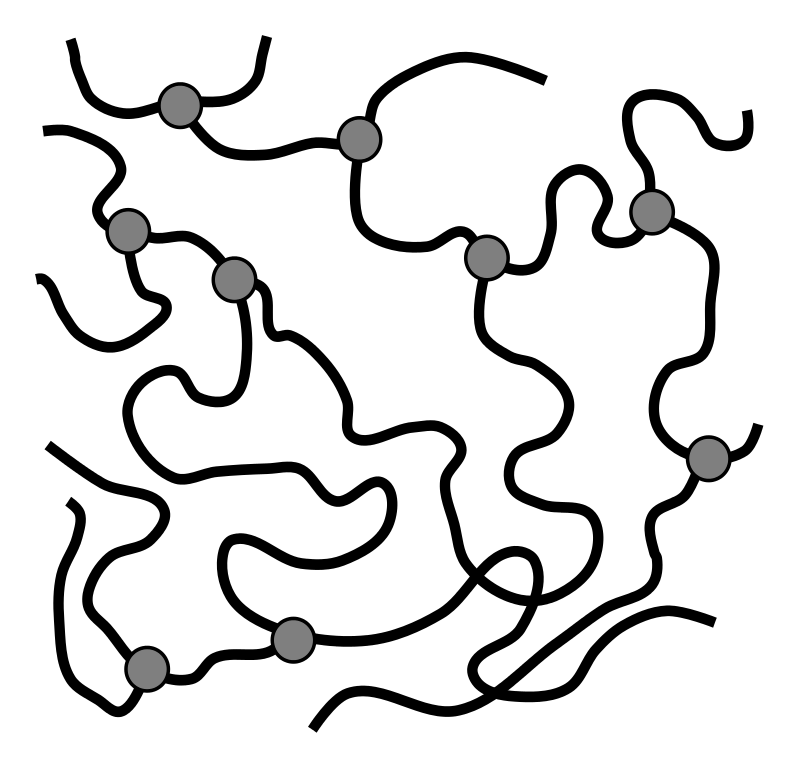
\includegraphics[width=0.25\textwidth]{chap1/include/figures/microstructure/microstructure-4.png}\\
\small (a) Amorphous. & \small (b) Semi-crystaline. & \small (c) Slightly cross-linked. & \small (d) Highly cross-linked.
\end{tabular}
\caption{Typical microscopic structures of polymers.}
\label{chap1:fig:polymer_processing_microstructure}
\end{figure}

\subsection{Extrusion process}
\label{chap1:subsec:polymer_processing_extrusion_process}

Several manufacturing technologies are used in the polymer processing industry to process thermoplastics, which mainly depend on the characteristics of the desired product, particularly on its geometry.
Standard manufacturing technologies include the extrusion (pushing the molten polymer through a die), the injection moulding (injecting the molten polymer into a cavity), the extrusion blow moulding (inflating a molten polymer tube inside a mould to create a hollow part), the 3D printing (depositing a molten polymer layer by layer to form the part), and the thermoforming (using suction to force a heated polymer sheet into a mould).
A comprehensive literature on these manufacturing technologies and their application is found in M.G. McGrum et al., 1997~\cite{chap1:1997mccrum}, D.M. Bryce, 1997--1999~\cite{chap1:1996abryce,chap1:1997bryce,chap1:1998bryce,chap1:1999bryce}, T.A. Osswald et al., 2006~\cite{chap1:2006osswald}, Z. Tadmor et al., 2006~\cite{chap1:2006tadmor}, S. Thomas et al., 2009~\cite{chap1:2009thomas}, O.S. Carneiro et al., 2012~\cite{chap1:2012carneiro}, and D.G. Baird et al., 2014~\cite{chap1:2014baird}.
In the present work, a particular focus is provided for the extrusion process, which has a relevant role in nowadays polymer processing industry.

Constant cross-section items, such as tubing, sheets, films, and also structural components, such as profiles for window frames, are usually manufactured by extrusion.
An illustration of a typical thermoplastic profile extrusion line is provided in Figure~\ref{chap1:fig:polymer_processing_extrusion_line}.
The process is continuous and consists of an extruder, which comprises a screw rotating inside a heated barrel, and is gravity-fed with thermoplastic pellets from a top-mounted hopper, placed at the rear.
The rotating screw compresses and forces the raw polymeric material to move forward through the barrel, in which several independently controlled heating units, mounted in sequence, gradually increase the temperature necessary for the melting.
The viscous dissipation is another important thermodynamic phenomenon, responsible for generating the heat required to melt the polymer.
However, it makes more difficult the temperature control and increases the risk of overheating.
The extrusion die is mounted at the front of the barrel, and its cross-section corresponds to the desired product cross-section, through which the molten polymeric material, subject to compression, is forced to flow.

\begin{sidewaysfigure}
\centering
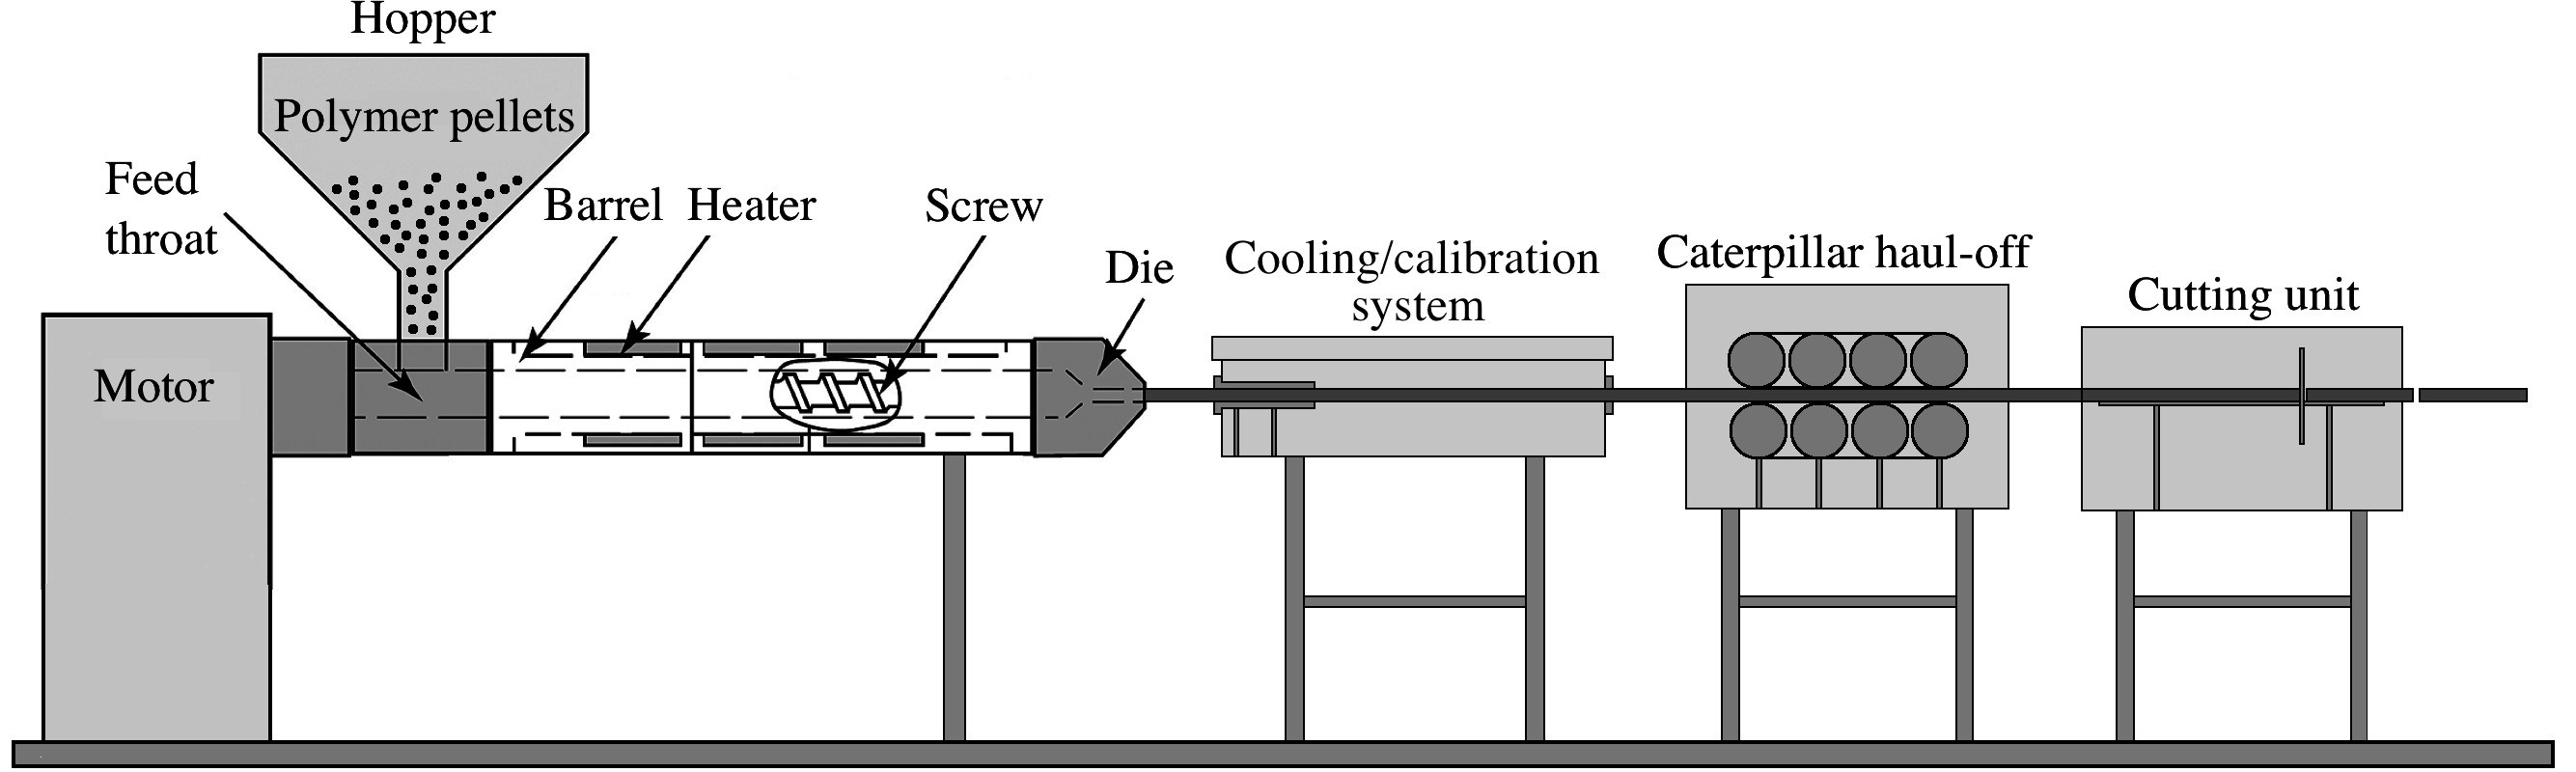
\includegraphics[width=1.0\textwidth]{chap1/include/figures/extrusion_line.png}
\caption[Typical thermoplastic profile extrusion line.]{Typical thermoplastic profile extrusion line (adapted from C. Rauwendaal, R. Gonzalez-Nunez, D. Rodrigue,
Polymer processing: extrusion, in Encyclopedia of polymer science and technology, John Wiley \& Sons, 2017).}
\label{chap1:fig:polymer_processing_extrusion_line}
\end{sidewaysfigure}

After leaving the extrusion die, the still molten product is cooled and geometrically calibrated to guarantee the desired shape on the solidified product.
Pipes are usually cooled with chilled water baths inside sealed chambers subject to a carefully controlled vacuum that avoids the molten polymer from collapsing or deforming, before solidification.
Other profiles, such as structural components, are usually cooled in contact with metallic systems, having an internal chilled water system, which also calibrates the product relevant dimensions, as illustrated in Figure~\ref{chap1:fig:polymer_processing_calibrator}.
Subsequently, a caterpillar haul-off, composed of puller rolls, imposes the desired linear production velocity to the extruded product.
A typical extrusion line ends with a cutting unit, which cuts the profile into predefined lengths.

\begin{figure}[!htb]
\centering
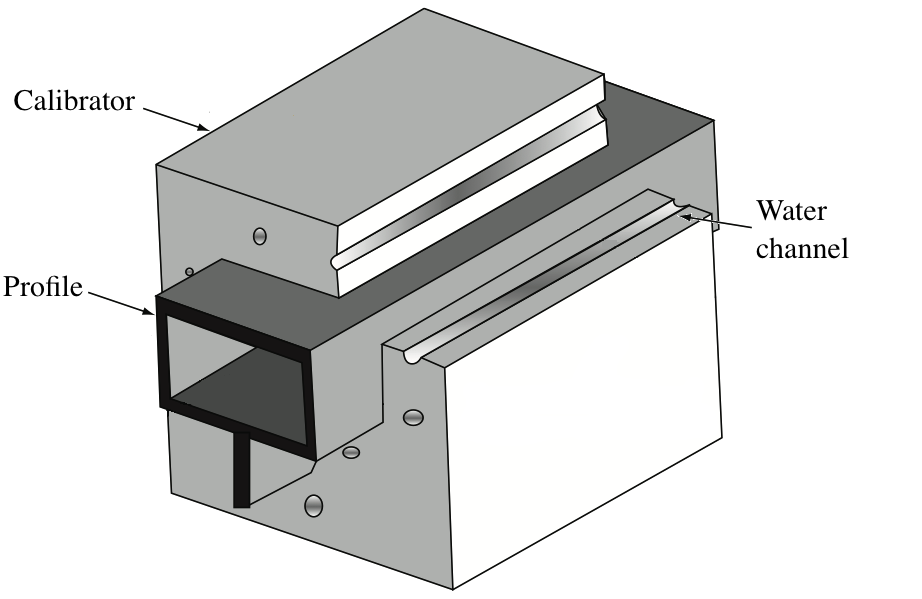
\includegraphics[width=0.65\textwidth]{chap1/include/figures/calibrator1.png}
\caption[Example of a cooling/calibrator system for the thermoplastic profile extrusion.]{Example of a cooling/calibrator system for the thermoplastic profile extrusion (adapted from O.S. Carneiro, J.M. N\'obrega, Design of extrusion forming tools, Smithers Rapra, Shawbury, 2012).}
\label{chap1:fig:polymer_processing_calibrator}
\end{figure}

\subsection{Industrial challenges}
\label{chap1:subsec:polymer_processing_industrial_challenges}

Polymer processing industries are highly sophisticated with advanced, expensive, and highly-automated manufacturing technologies.
However, the complex behaviour of polymers and the complex thermo-mechanical processes involved in these manufacturing technologies, raise challenging engineering problems, even for experienced polymer engineers.
Some of these challenges in the case of the extrusion are described hereafter.

The flow balance of the molten polymeric material at the die openings is crucial to avoid that more material flows through the thicker sections of the profile, when compared with the thinner ones~\cite{chap1:2017rajkumar}.
Therefore, an unbalanced flow does not allow to obtain the shape desired for the final solidified product, as exemplified in Figure~\ref{chap1:fig:polymer_processing_extrusion_deffects} for the case of a deck.
The usual practice to ensure a balanced flow consists in gradually adjusting the die geometry from the barrel to the openings, such that the thinner sections of the profile are compensated with more material.
However, due to the complex behaviour of the molten polymeric material, the effect of these adjustments in the flow is difficult to predict through pure analytic approaches mainly due to the large number of variables involved in the process.
On the other side, the common trial-and-error approach requires large amounts of resources, is very time-consuming, and might limit the possibility to achieve optimal configurations.
Indeed, the die design is a challenging task, even for experienced polymer engineers, leading to increased costs.

\begin{figure}[!htb]
\centering
\begin{tabular}{@{}c@{\hskip 1.5cm}c@{}}
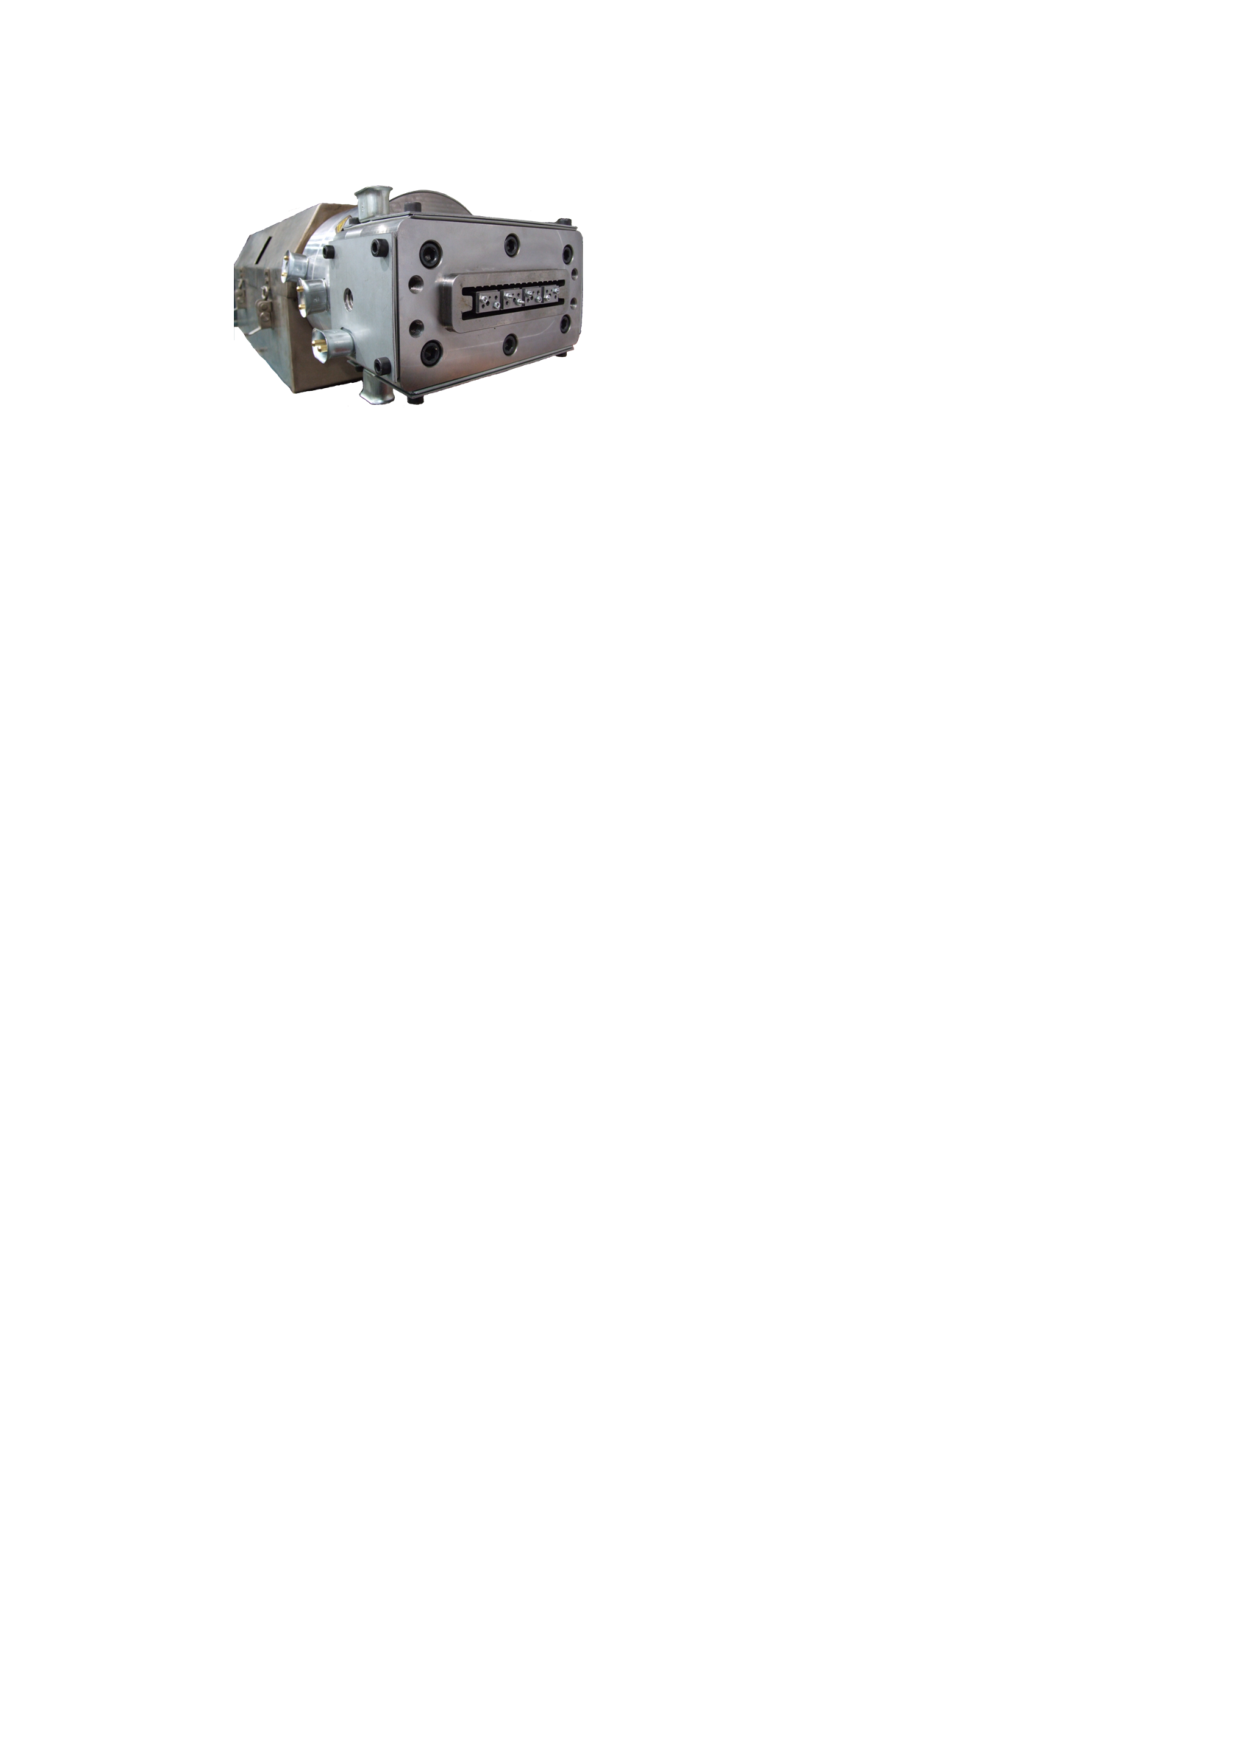
\includegraphics[width=0.4\textwidth]{chap1/include/figures/extrusion_die.pdf}
& 
\includegraphics[width=0.3\textwidth]{chap1/include/figures/deck.pdf}\\
\small (a) Extrusion die. & \small (b) Defective profile.
\end{tabular}
\caption[Extrusion die for the production of deck and defective profile resulted from an unbalanced flow.]{Extrusion die for the production of deck and defective profile resulted from an unbalanced flow (adapted from L. Ferr\'as, Theoretical and numerical studies of slip flows, PhD Thesis, Universidade do Minho, 2012).}
\label{chap1:fig:polymer_processing_extrusion_deffects}
\end{figure}

Another challenge of great concern in the extrusion, which also applies other different manufacturing technologies, is the cooling of the molten polymeric material after leaving the die~\cite{chap1:2017rajkumar}.
The cooling rate strongly determines the structure of the polymeric material and, thus, affects the physical properties of the final solidified product, such as density, optical and barrier properties, coefficient of friction, and impact behaviour.
In that regard, a high cooling rate is usually desired, particularly in the case of sheets and films, avoiding large crystallites and, consequently, providing smoothness and transparency.
Moreover, fast cooling is also desired for increasing the production and profitability of the process.
On the other side, the average temperature on the profile cross-section must fall below the solidification point of the polymeric material after the cooling stage.
Unfortunately, a high cooling rate might result in solidified borders and molten cores, especially in thicker sections, which might induce subsequent remelting of the product due to heat conduction.
Moreover, different cooling rates result in internal residual stresses, which also lead to subsequent deformation of the final solidified product.
In that regard, a uniform cooling rate is desired across the profile cross-section, which in general conflicts with a high cooling rate.

The previous challenge leads to an optimization problem, for which several parameters have to be considered, as illustrated in Figure~\ref{chap1:fig:polymer_processing_cooling_parameters}, namely, the extrusion conditions, cooling conditions, profile geometry, system geometry, polymer properties, metal properties (in the case of structural components), and the vacuum conditions (in the case of tubing and pipes), among others.
In the case of structural components, the optimization often consists in performing adjustments to the cooling/calibrator system geometry, configuration, or cooling conditions.
As in the previous case, the optimization problem is commonly performed with trial-and-error approaches implying the same drawbacks, which often leads to intractable challenges.
Similar challenges arise in the case of the injection moulding, where most of the residence time is dedicated to the cooling stage and, therefore, optimizing the heat transfer under the same principles is of crucial importance.

In light of the drawbacks of trial-and-error approaches in the context of these industry challenges, there is a deep concern for developing innovative and efficient alternative design approaches.
In that regard, the emerging field of computational modelling has received increasing attention from the industry side to provide means of overcoming these challenges and effectively support design activities.

\begin{figure}[!htb]
\centering
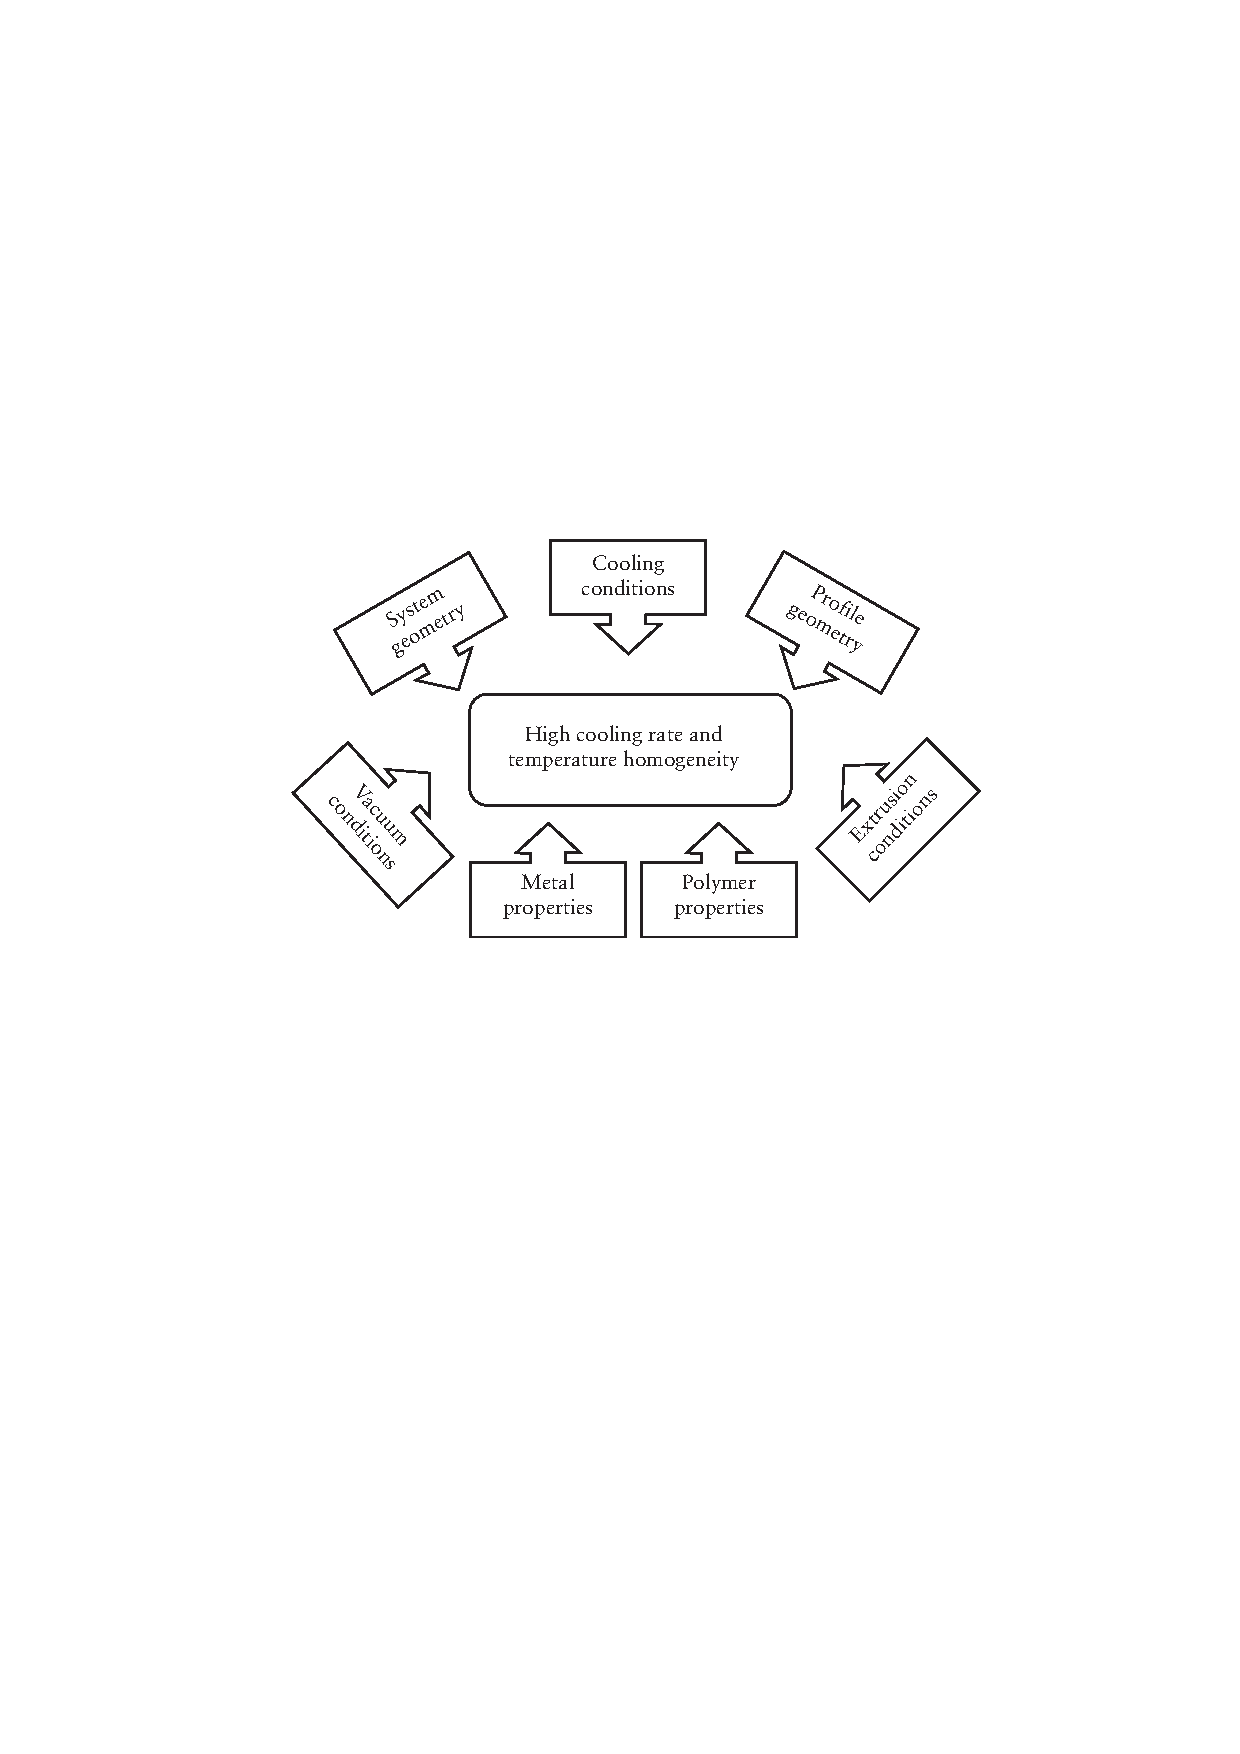
\includegraphics[width=0.7\textwidth]{chap1/include/figures/cooling_parameters.pdf}
\caption[Parameters affecting the optimization of the extrusion cooling stage.]{Parameters affecting the optimization of the extrusion cooling stage (adapted from O.S. Carneiro, J.M. N\'obrega, Design of extrusion forming tools, Smithers Rapra, Shawbury, 2012).}
\label{chap1:fig:polymer_processing_cooling_parameters}
\end{figure}

% end of file
